\section{Results}

We present results for three major settings:
\begin{itemize}
    \item Performance of fully pre-trained large language models across different number of shots.
    \item Development of performance over the course of training on our pre-training datamix.
    \item Scaling laws ablations across different compute flops and seeds.
\end{itemize}

\subsection{Performance on fully trained models}

We first consider the performance of fully pre-trained models from the Llama, Gemma, and Mistral series on 5 tasks - ANLI, HansNLI, MNLI, SNLI, and AbductiveNLI. The results are pictured in Figures \ref{fig:anli} - \ref{fig:abductivenli}. For all models, we observe the zero shot performance to be bad on all tasks except AbductiveNLI, but it improves with adding few shots in the prompt. Even with just one shot, the performance is significantly better than the zero shot accuracy. Adding more than three or four examples in the few shots does not improve performance much and saturates till 10 shots. As for comparison between different models, there's clear gap between the smaller and larger models. For example for the Llama series, 405B performs the best followed by 70B and then the 8B. Even though all three of them are trained on the same amount of text tokens, model performance clearly improves with scale. One exception is AbductiveNLI, where the 70B and 405B have similar performance around 85\%.

Another important thing to observe is the performance comparison with fine-tuned BERT. \citet{brown2020languagemodelsfewshotlearners} observed chance accuracies for GPT-3 models on the ANLI task. Even with scale and few shot examples, the performance only improved marginally. This might have been a factor in the community dropping NLI tasks as benchmarks for decoder-only models like GPT, Llama, Mistral, Gemma, etc. In our study, we observe performance of more capable models like Llama 405B to be on-par or better than the fine-tuned BERT performance, even though no training data from the NLI tasks is used during the pre-training of LLMs. The difference is clearly visible for ANLI and AbductiveNLI, where Llama-3.1 405B performances significantly better than fine-tuned BERT.

\begin{figure}[t]
    \centering
    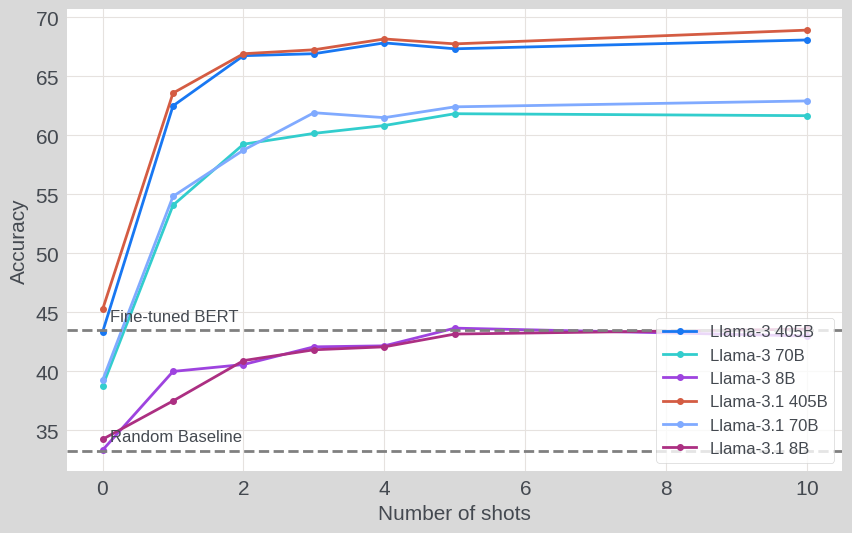
\includegraphics[width=0.45\textwidth]{nli_plots/anli.png}
    \caption{ANLI}
    \label{fig:anli}
\end{figure}

\begin{figure}[t]
    \centering
    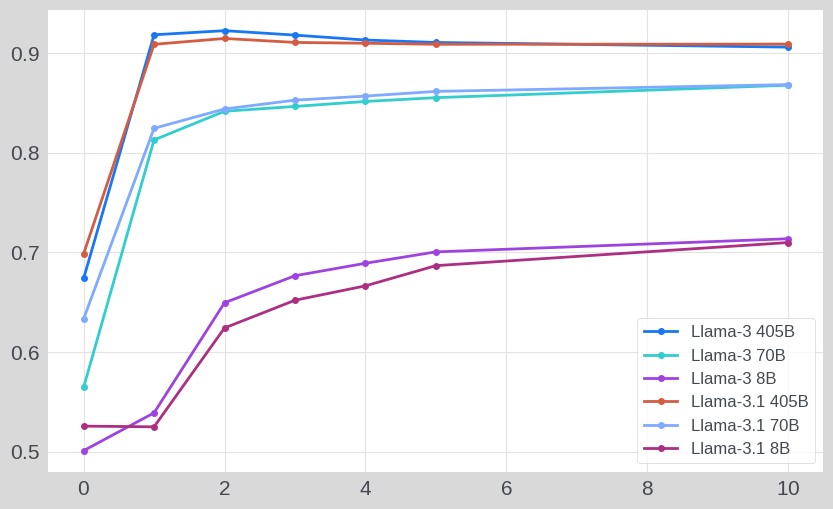
\includegraphics[width=0.45\textwidth]{nli_plots/hansnli.png}
    \caption{HansNLI}
    \label{fig:hansnli}
\end{figure}

\begin{figure}[t]
    \centering
    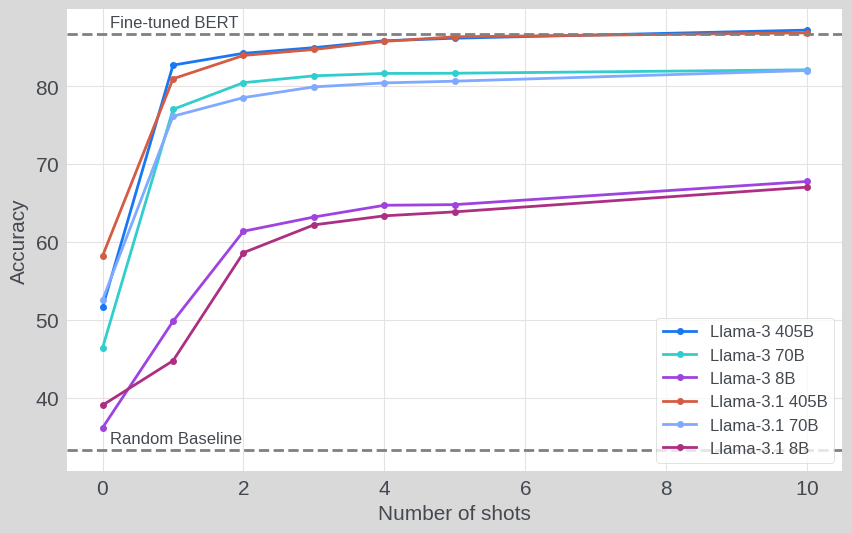
\includegraphics[width=0.45\textwidth]{nli_plots/mnli_matched.png}
    \caption{MNLI}
    \label{fig:mnli}
\end{figure}

\begin{figure}[t]
    \centering
    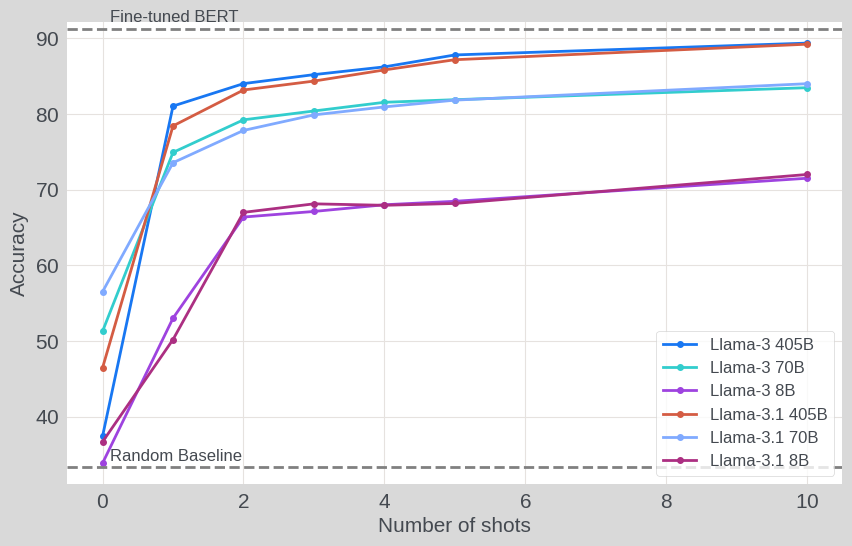
\includegraphics[width=0.45\textwidth]{nli_plots/snli.png}
    \caption{SNLI}
    \label{fig:snli}
\end{figure}

\begin{figure}[t]
    \centering
    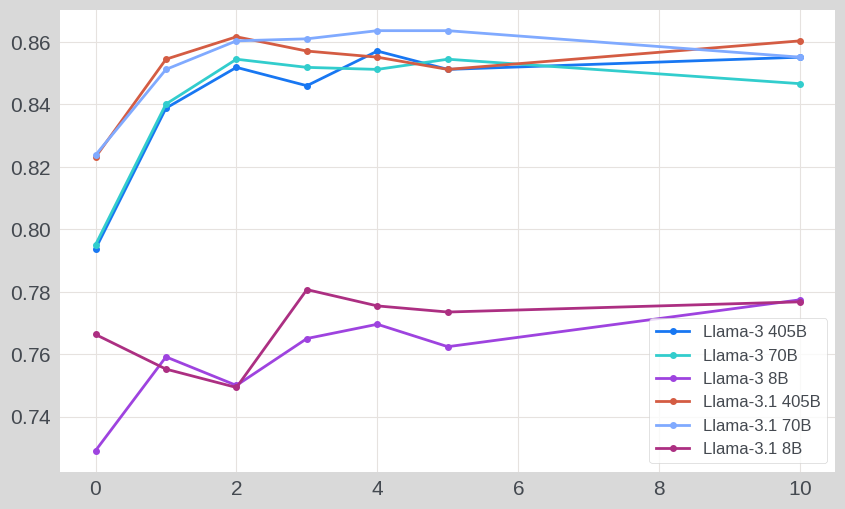
\includegraphics[width=0.45\textwidth]{nli_plots/abductivenli.png}
    \caption{AbductiveNLI}
    \label{fig:abductivenli}
\end{figure}

\subsection{Performance development over training}

We pre-train Llama-3 architecture based 8B and 70B models from scratch for 2T tokens. The details of the pre-training mix are provided in Appendix \ref{sec:appendix}. Plots for both the 8B and 70B models pre-trained from scratch are depicted in Figures \ref{fig:anli_int} - \ref{fig:abductivenli_int}. We depict the 4-shot performance for all tasks as most models saturate around four shots on each of the tasks. We observe that the 70B model starts improving quickly after around training on around 250B tokens. For the ANLI and AbductiveNLI tasks, it crosses fine-tuned BERT performance around 500B tokens. On the other hand, the development of performance for the 8B model is very slow, and stays around chance accuracy for HansNLI, MNLI, and SNLI. From the final model performance of 8B depicted in Figures \ref{fig:anli} - \ref{fig:abductivenli}, we can conclude that the 8B model improves fairly late during the training stage. We did not have the budget to do the full pre-training run, but longer training definitely seems to help on NLI tasks.

Additionally, following \citet{variancepaper}, we compute monotonicity on both discrete and continuous metrics for the model pre-training in Table \ref{tab:monotonicity}. Tracking continuous metrics like negative log likelihood (NLL) over the course of the training is in general better compared to discrete metrics like accuracy. We use the NLL of the target answer and accuracy as the continuous and discrete metric respectively.

\begin{table*}
\centering
\begin{tabular}{|l|cc|cc|}
    \hline
    Model $\rightarrow$ & \multicolumn{2}{c|}{8B} & \multicolumn{2}{c|}{70B} \\
    \hline
    Benchmark $\downarrow$ & $mon_{disc}$  & $mon_{cont}$ & $mon_{disc}$ & $mon_{cont}$ \\
    \hline
    AbductiveNLI & 0.623 & 0.618 & 0.79 & 0.793 \\
    \hline
    ANLI & - & - & 0.67 & 0.474 \\
    \hline
    HansNLI & 0.316 & 0.457 & 0.57 & 0.629 \\
    \hline
    MNLI & 0.335 & 0.507 & 0.772 & 0.798 \\
    \hline
    SNLI & 0.051 & 0.382 & 0.637 & 0.651 \\
    \hline
    \end{tabular}
\caption{Monotonicity values for the 8B and 70B models during the course of the training. We report both the discrete ($mon_{disc}$) and continuous ($mon_{cont}$) monotonicity values.}
\label{tab:monotonicity}
\end{table*}

\begin{figure}[t]
    \centering
    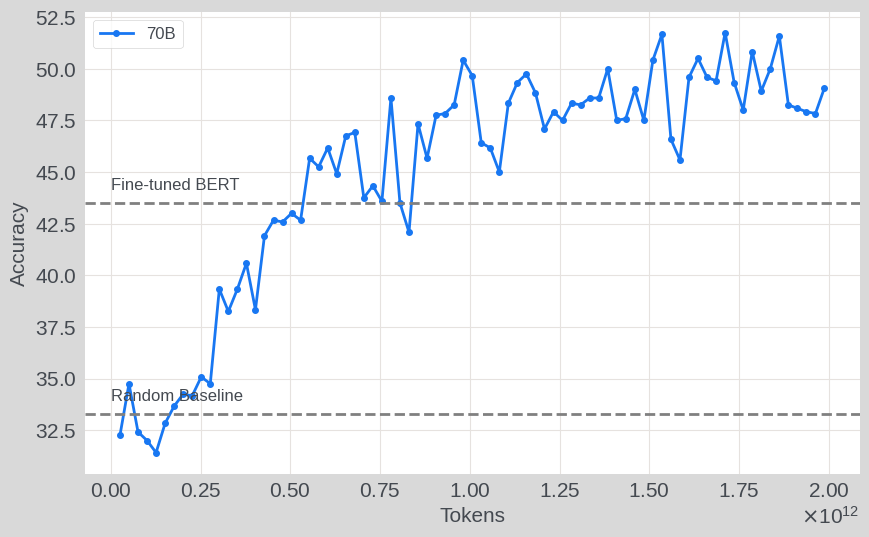
\includegraphics[width=0.45\textwidth]{nli_plots/anli_intermediate.png}
    \caption{ANLI}
    \label{fig:anli_int}
\end{figure}

\begin{figure}[t]
    \centering
    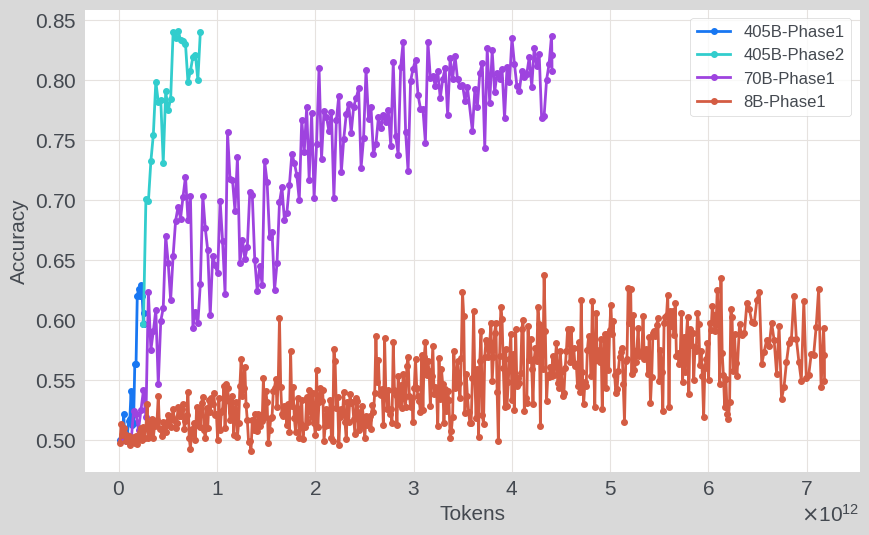
\includegraphics[width=0.45\textwidth]{nli_plots/hansnli_intermediate.png}
    \caption{HansNLI}
    \label{fig:hansnli_int}
\end{figure}

\begin{figure}[t]
    \centering
    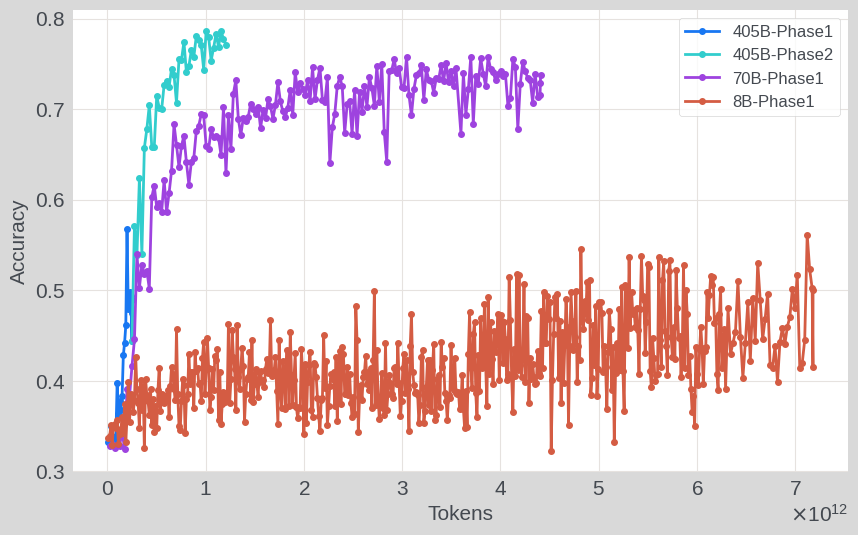
\includegraphics[width=0.45\textwidth]{nli_plots/mnli_matched_intermediate.png}
    \caption{MNLI}
    \label{fig:mnli_int}
\end{figure}

\begin{figure}[t]
    \centering
    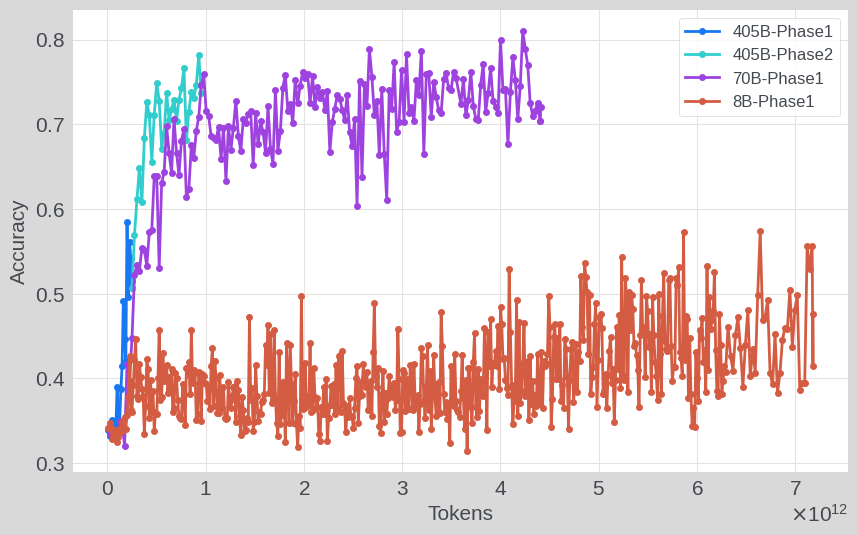
\includegraphics[width=0.45\textwidth]{nli_plots/snli_intermediate.png}
    \caption{SNLI}
    \label{fig:snli_int}
\end{figure}

\begin{figure}[t]
    \centering
    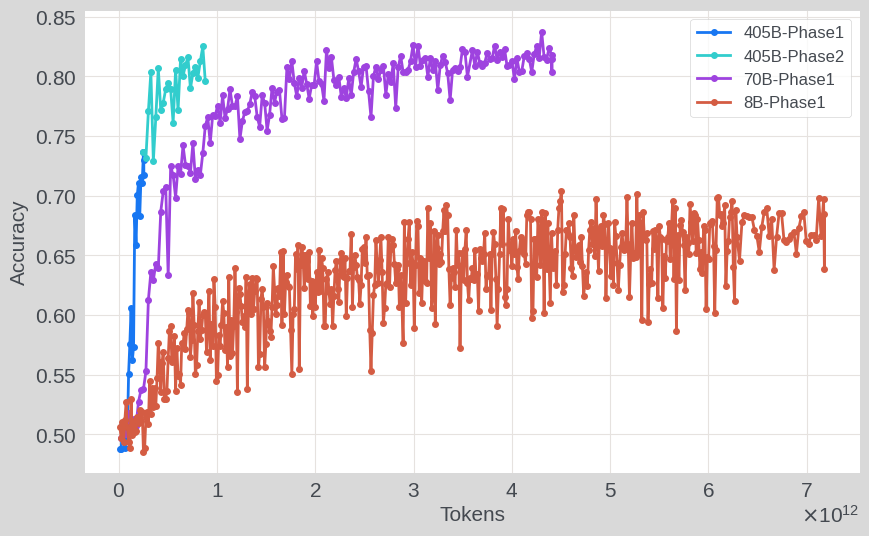
\includegraphics[width=0.45\textwidth]{nli_plots/abductivenli_intermediate.png}
    \caption{AbductiveNLI}
    \label{fig:abductivenli_int}
\end{figure}

\begin{figure*}[ht]
    \centering
    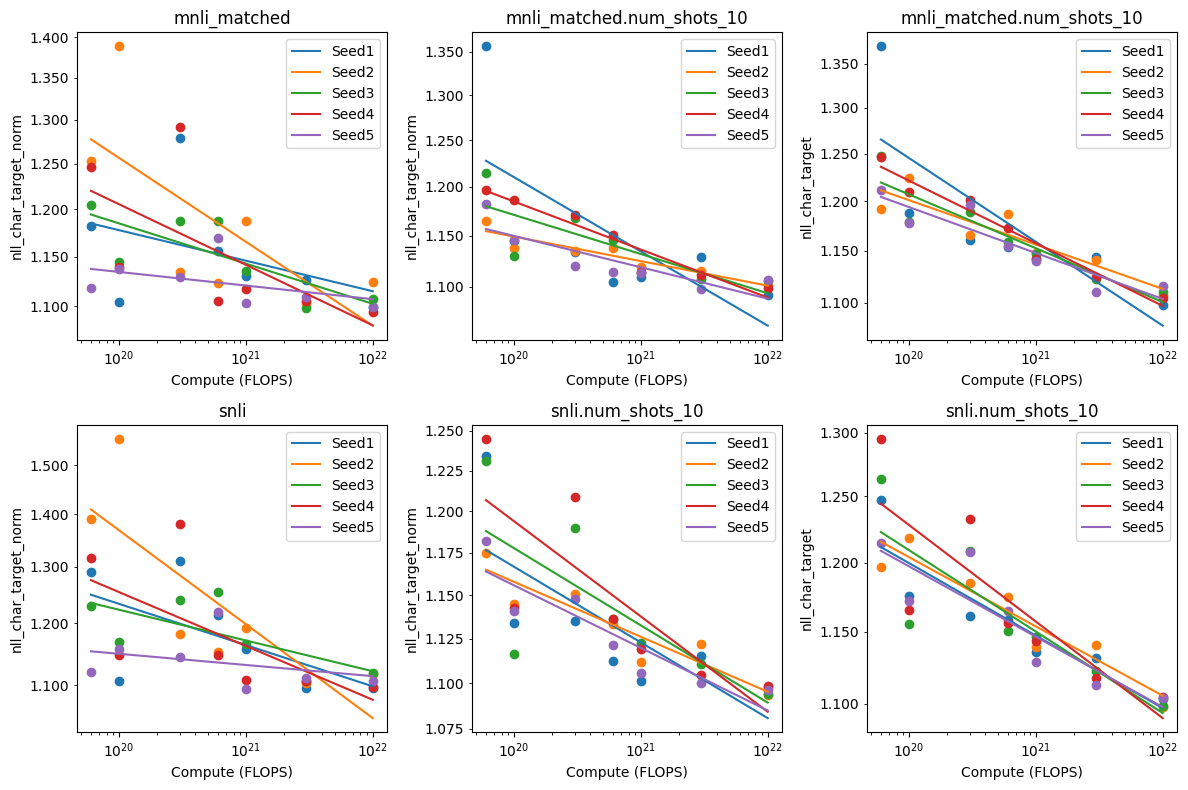
\includegraphics[width=0.95\textwidth]{nli_plots/sl_fits_mnli_snli.png}
    \caption{Scaling law curve fits across different compute FLOPs}
    \label{fig:sl_mnli_snli}
\end{figure*}

\paragraph{Q1: Does NLI provide signal for LLMs?}
We show \begin{enumerate}
    \item curves + scores on trained-out models.  Conclusion: ? Should say something about whether it is separating models in early stages of training, and whether it is monotonic, how much variance etc.
    \item Trained out model scores. Tentative conclusion (pending numbers): with the exception of abductive NLI, these datasets allow to distiguish models of different sizes. Doesn't work at all with zero-shot (which can explain some previous results?), but with one or two shots we get decent scores. ANLI seems to be the most challenging with around 70\% accuracy on the 405B model.
    \item Ablations: conclusion??
\end{enumerate}

\section{Analysis with ChaosNLI}

\citet{nie-etal-2020-learn} release the ChaosNLI dataset, which is comprised of human annotations for a subset of MNLI, SNLI, and AbductiveNLI. They collect 100 human annotations for 3113 samples for MNLI and SNLI, and 1532 samples in AbductiveNLI. In this section, we analyse the performance of models with respect to the majority labels and entropy of the label distribution according to the human annotators.

We look at the probability distribution according to the models over the three labels (\textit{Entailment}, \textit{Neutral}, and \textit{Contradiction}) and compute the Jensen-Shannon Divergence (JSD) \citep{menendez1997jensen} over the softmax probability distribution and human annotator distribution of the labels. Mathematically, JSD is defined as:

\begin{equation}
    \scriptstyle JSD(p || q) = \sqrt{\frac{1}{2}KL(p || m) + \frac{1}{2}KL(q || m)}
\end{equation}

where $p$ is the human annotator distribution, $q$ is the softmax probability distribution, and $m = \frac{1}{2}(p + q)$. The benefit of using JSD over KL divergence is that it is symmetric and bounded between 0 and 1.

\begin{figure*}
    \centering
    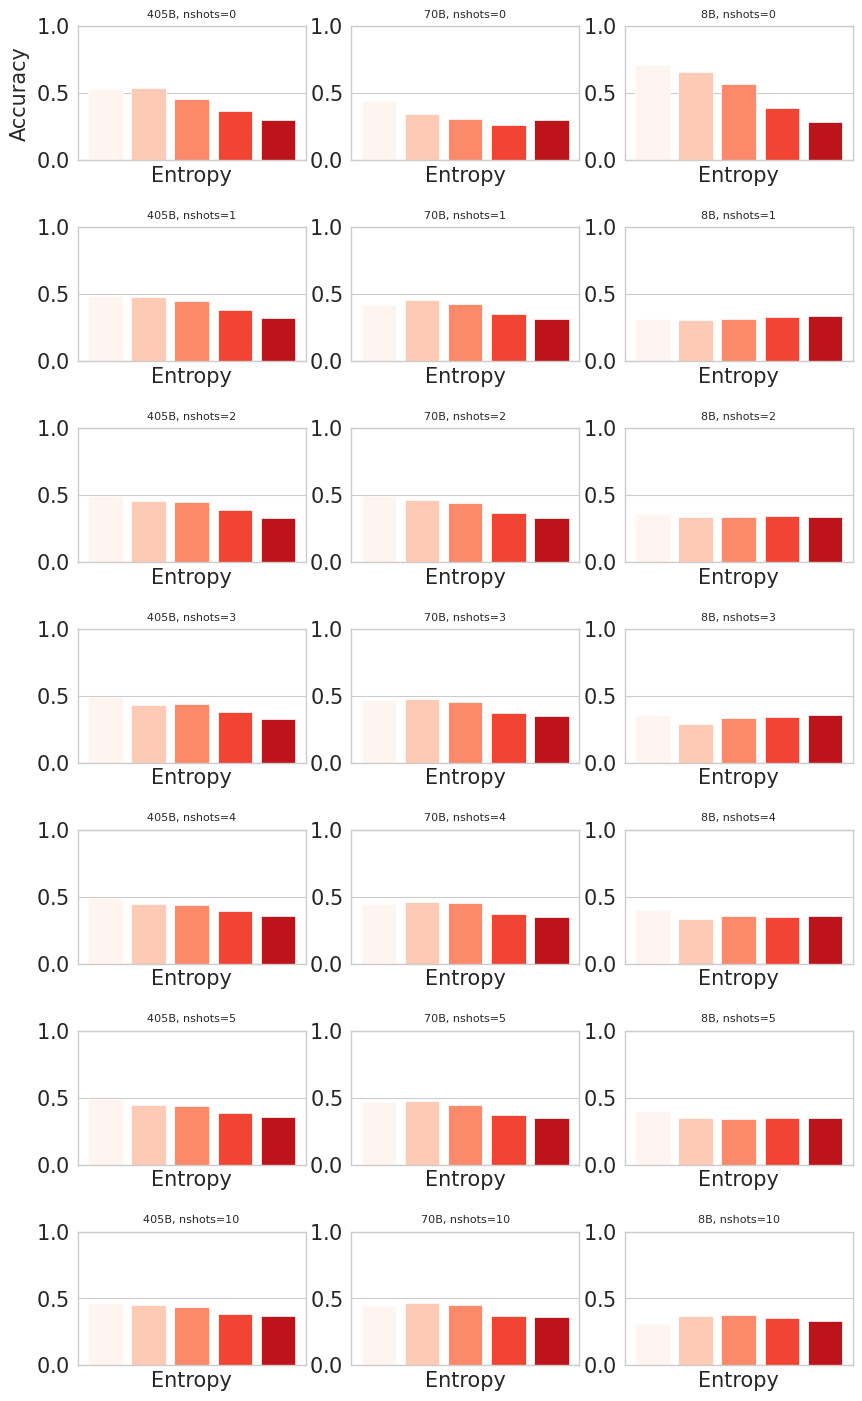
\includegraphics[width=0.98\linewidth]{nli_plots/mnli_matched_entropy_acc.png}
    \caption{Accuracy vs entropy plots for MNLI}
    \label{fig:entropy_accuracy_mnli}
\end{figure*}

NB: put contamination results somewhere.

Overall conclusion: seems to be useful both for training and trained-out models, an open question however is, is there still room to improve?

\paragraph{Q2: Is there still room for improvement?}
We do an light-weight manual analysis (e.g. check 20 examples).
Probable conclusion: there may be some errors, but oftentimes models make incorrect predictions on samples on which humans may disagree too.

To substantiate this claim, we consider chaosNLI.
We show 1) entropy plots for various models, these show that the larger models have pretty much perfect perfrmance on samples where humans agree across the board, but drop off on other examples. Smaller models don't get perfect performance also on the former. Results also show that a small amount of errors is due to annotation errors (or not matching majority labels), because the `corrected' accuracy is slightly higher than the non-corrected accuracy.
2) We show KL-divergence with human distributions. Conclusion: this gets better with scale (contradicts earlier findings!), but still far away from human alignment. Still room for improvement. We check how stable this signal is across training (so we show curves of KL/JSD and see whether this provides a astable signal.


% \begin{itemize}
%   \item Final pre-trained model result analysis. How model size, prompts, and shots affect things across various tasks.
%   \item Development of model performance for a given task across model sizes.
%   \item Correlation of model performance development with other commonsense/normal reasoning tasks (race, obqa, mmlu, math, etc.)
%   \item Results on ChaosNLI and how model scores relate to the distribution of human judgements. Model size/prompt analysis for this too.
%   \item Large models are good, but is it because of better models/training or just contamination? Contamination Analysis on various benchmarks.
%   \item Can NLI tasks help in pre-training ablations? Results on seed models and models trained on different datamixes. How does the effectiveness of a given dataset/datamix is affected under different datasets (both commonsense reasoning and standard datasets).
% \end{itemize}
